
\section{Non-Serializable Execution Counterexample}
\label{appendix:non-serializable-execution-example}

%\medskip
%\noindent
%\textbf{Serializable NFA Extraction.}
%%
%
%
%
%\begin{wrapfigure}{r}{0.5\textwidth}  % “r” = right, width = 0.5\textwidth
%	\centering
%	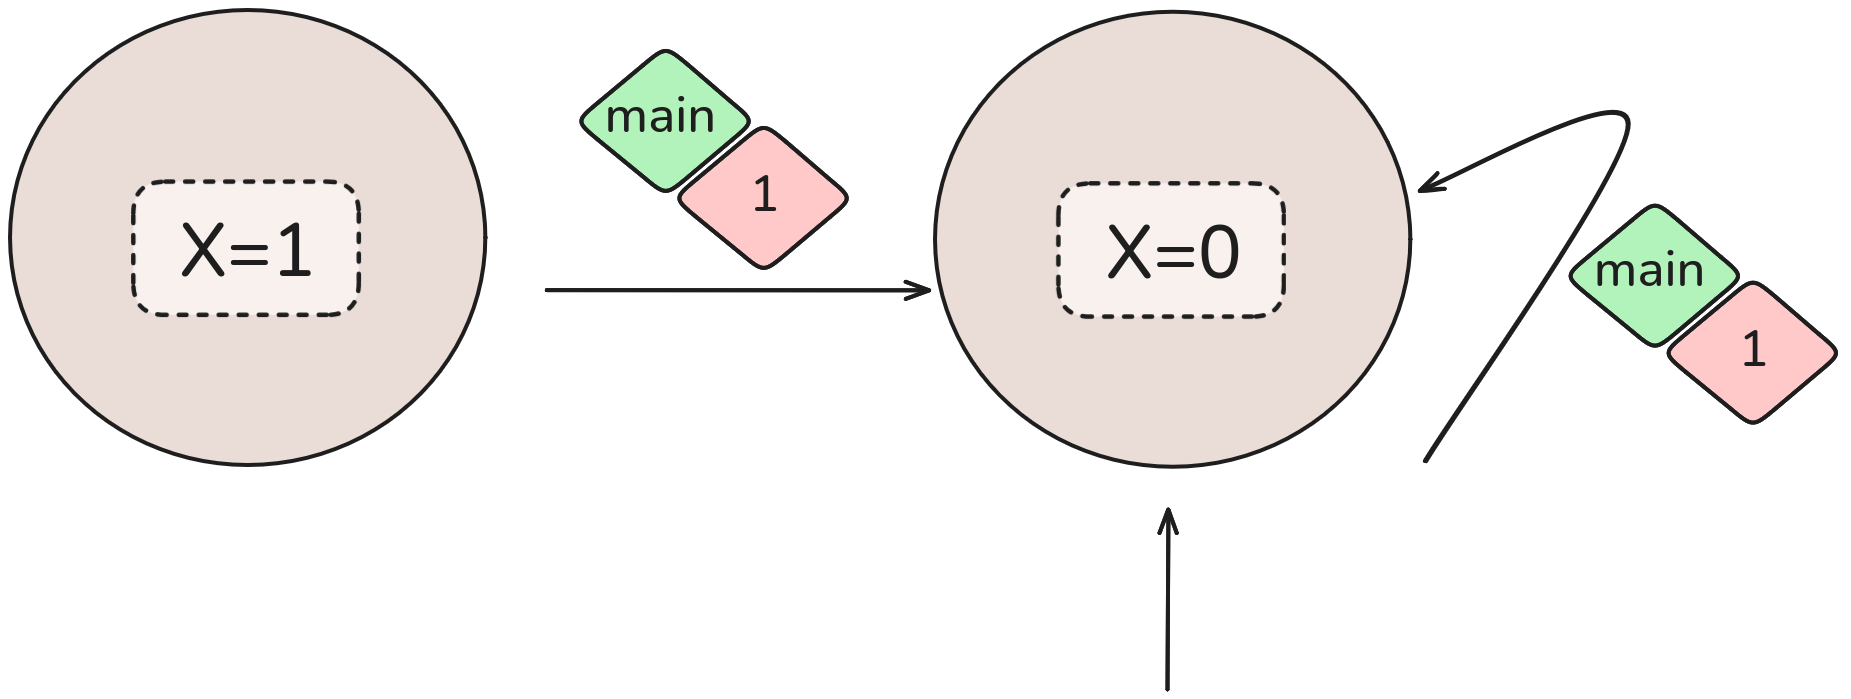
\includegraphics[width=0.48\textwidth,trim=0 0 0 0,clip]{plots/code_2_NFA.png}
%	\caption{NFA for serialized executions of Listing~\ref{lst:MotivatingExample2NonSer}.}
%	\label{fig:code2ExampleNFA}
%\end{wrapfigure}

%\begin{figure}[!htbp]
%	\centering
%	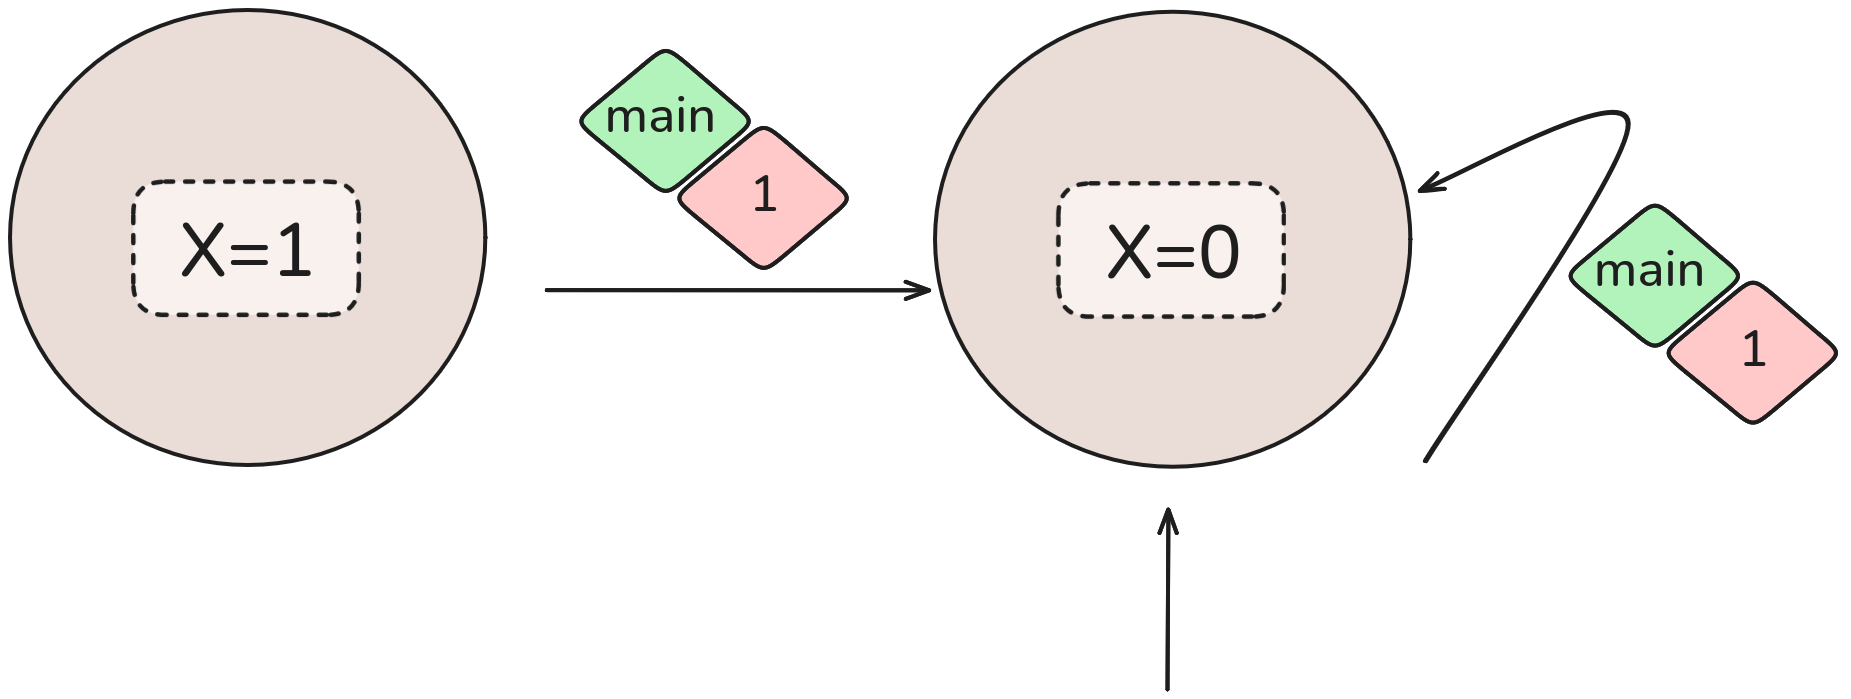
\includegraphics[width=0.5\textwidth,trim=0 0 0 0,clip]{plots/code_2_NFA.png}
%	\caption{NFA for serialized executions of Listing~\ref{lst:MotivatingExample2NonSer}.}
%	\label{fig:code2ExampleNFA}
%\end{figure}
%
%\medskip
%\noindent
%\textbf{Petri Net Extraction.}
%
%
%
%\medskip
%\noindent
%\textbf{Counterexample Extraction.}
%%
%
%%


\begin{table}[!htbp]
	\centering
	\label{tab:reach-seq}
	\resizebox{0.9\textwidth}{!}{
		\begin{tabular}{c l c c c c c c}
			\toprule
			\textbf{Step} 
			& \textbf{Firing} 
			& \multicolumn{3}{c}{\textbf{Marking (after firing)}} 
			& \multicolumn{3}{c}{\textbf{Description (after firing)}} \\
			\cmidrule(lr){3-5} \cmidrule(lr){6-8}
			& 
			& \textbf{Global} 
			& \textbf{Local} 
			& \textbf{Responses} 
			& \textbf{Global state} 
			& \textbf{In-flight requests} 
			& \textbf{Responses} \\
			\midrule
			0 & --                                  
			& {\color{blue}$P_3$(1)}                  
			& --                                    
			& --                                    
			& {\color{blue}[X=0]}                   
			& --                          
			& --                                    \\
			1 & $t_1$ 
			& {\color{blue}$P_3$(1)}                  
			& $P_1$(1)                                
			& --                                    
			& {\color{blue}[X=0]}                   
			& {\color{ForestGreen}$\blacklozenge_\text{main}$} 
			& --                                    \\
			2 & $t_1$ 
			& {\color{blue}$P_3$(1)}                  
			& $P_1$(2)                                
			& --                                    
			& {\color{blue}[X=0]}                   
			& {\color{ForestGreen}$\blacklozenge_\text{main}$}, {\color{ForestGreen}$\blacklozenge_\text{main}$}  
			& --                                    \\
			3 & $t_3$                                  
			& {\color{blue}$P_2$(1)}                  
			& $P_1$(1),$P_4$(1)                          
			& --                                   
			&                                    {\color{blue}[X=1]}    
			&                                    {\color{black}$\blacklozenge_\text{until yield}$}, {\color{ForestGreen}$\blacklozenge_\text{main}$}   
			& --                                    \\
			4 & $t_2$                                  
			& {\color{blue}$P_2$(1)}                  
			& $P_4$(2)                                
			& --                                    
			&                                    {\color{blue}[X=1]}    
			&                                    {\color{black}$\blacklozenge_\text{until yield}$}, {\color{black}$\blacklozenge_\text{until yield}$}   
			& --                                    \\
			5 & $t_4$                                  
			& {\color{blue}$P_3$(1)}                  
			& $P_5$(1),$P_4$(1)                          
			& --                                    
			&                                   {\color{blue}[X=0]}     
			&                                    {\color{black}$\blacklozenge_\text{after yield}$}, {\color{black}$\blacklozenge_\text{until yield}$}   
			& --                                    \\
			6 & $t_6$                     
			& {\color{blue}$P_3$(1)}                  
			& $P_4$(1)                                
			& {\color{red}$P_7$(1)}                    
			&                                      	{\color{blue}[X=0]}  
			&                                    {\color{black}$\blacklozenge_\text{until yield}$}   
			&                                   {\color{red}$\blacklozenge_1$}     \\
			7 & $t_5$                                  
			& {\color{blue}$P_3$(1)}                  
			& $P_6$(1)                                
			& {\color{red}$P_7$(1)}                    
			&                                   {\color{blue}[X=0]}    
			&                                    {\color{black}$\blacklozenge_\text{after yield}$}      
			&                                   {\color{red}$\blacklozenge_1$}        \\
			8 & $t_7$                     
			& {\color{blue}$P_3$(1)}                                  
			& --                                    
			& {\color{red}$P_7$(1),\color{red}$P_8$(1)}    
			&                                   {\color{blue}[X=0]}    
			&                                   --    
			&                                   {\color{red}$\blacklozenge_0$}, {\color{red}$\blacklozenge_1$}       \\
			\bottomrule
		\end{tabular}
	}
	\caption{The firing sequence reaching marking $M^*$ which is in our target semilinear set. The marking $P_i(n_j)$ indicates that there are $n_j$ tokens on place $P_i$. The initial marking has a single token in place $P_3$ encoding $g_0$.}
	\label{tab:PetriNetFiringCounterexample}
\end{table}

%\newpage
